%==============================================================
%  CityVision — Preuve de concept : EoMT face à la baseline
%  20 diapositives (≈ 20 min). Notes orales : \note{...} de chaque diapositive.
%
%  Compilation (dans ce dossier, 2 passes pour la numérotation) :
%      pdflatex cityvision_poc.tex
%      pdflatex cityvision_poc.tex
%  Notes à l'écran : décommenter \setbeameroption{show notes on second screen=right}
%  Images : dossier img/
%==============================================================
\documentclass[aspectratio=169,9pt,xcolor=table,t]{beamer}

\usepackage[utf8]{inputenc}
\usepackage[T1]{fontenc}
\usepackage[french]{babel}
\usepackage{lmodern}
% Ponctuation française écrite explicitement (~: ~; ~?) : les raccourcis actifs de
% babel cassent TikZ/pgfplots dans les diapositives Beamer.
\AtBeginDocument{\shorthandoff{;:!?}}

\usepackage{amsmath,amssymb,bm,dsfont}
\usepackage{booktabs,tabularx,array}
\usepackage{graphicx}
\usepackage{tikz}
\usetikzlibrary{arrows.meta,positioning,calc,babel}
\usepackage{pgfplots}
\pgfplotsset{compat=1.18}
\usepackage[most]{tcolorbox}
\usepackage{ragged2e}
% Texte aligné à gauche, sans césure (colonnes et blocs compris)
\AtBeginDocument{\RaggedRight\hyphenpenalty=10000\exhyphenpenalty=10000}
\AtBeginEnvironment{column}{\RaggedRight}

% \setbeameroption{show notes on second screen=right}

% ---- Palette ------------------------------------------------
\definecolor{navy}{HTML}{15202E}      % texte, fonds sombres
\definecolor{paper}{HTML}{F6F5F1}     % fond clair
\definecolor{paper2}{HTML}{EBEEF1}    % second fond clair
\definecolor{bodyc}{HTML}{4A5568}     % texte courant
\definecolor{mutedc}{HTML}{6A7380}    % pied de page
\definecolor{accent}{HTML}{0F7B5F}    % surtitres
\definecolor{mint}{HTML}{5FD3A8}      % accent sur fond sombre
\definecolor{paleblue}{HTML}{B8C4D0}  % texte secondaire sur fond sombre
\definecolor{palegrey}{HTML}{D7DEE5}
\definecolor{linec}{HTML}{DDE1E5}
\definecolor{cellgrey}{HTML}{D4D9DE}
\definecolor{softgrey}{HTML}{E4E8EC}
% une couleur par modèle (comme dans le dashboard)
\definecolor{cvblue}{HTML}{2A78D6}    % ResNet50-UNet
\definecolor{cvorange}{HTML}{EB6834}  % Mask2Former
\definecolor{cvgreen}{HTML}{1BAF7A}   % EoMT
\definecolor{dkblue}{HTML}{1D5BA8}
\definecolor{dkorange}{HTML}{B5430E}
\definecolor{dkgreen}{HTML}{0B2E22}
\definecolor{orangetint}{HTML}{FDF0E8}
\definecolor{greentint}{HTML}{E6F6EF}

% ---- Thème ---------------------------------------------------
\setbeamertemplate{navigation symbols}{}
\setbeamercolor{background canvas}{bg=paper}
\setbeamercolor{normal text}{fg=navy}
\setbeamercolor{structure}{fg=navy}
\setbeamercolor{itemize item}{fg=bodyc}
\setbeamercolor{enumerate item}{fg=navy}
\setbeamertemplate{itemize items}{\textbullet}
\setbeamertemplate{enumerate items}[default]
\setbeamersize{text margin left=10mm,text margin right=10mm}

\newcommand{\cvsource}{}
\newcommand{\setsource}[1]{\gdef\cvsource{\ \textperiodcentered\ #1}}

\setbeamertemplate{frametitle}{%
  \vspace*{2.5mm}%
  {\fontsize{6.5}{8}\selectfont\bfseries\color{accent}\MakeUppercase{\insertframesubtitle}}\par\vspace{0.8mm}%
  {\fontsize{17}{20}\selectfont\bfseries\color{navy}\insertframetitle}\par\vspace{1mm}}
\setbeamertemplate{footline}{%
  \hspace*{10mm}{\fontsize{6}{7}\selectfont\color{mutedc}CityVision \textperiodcentered\ Preuve de concept
  \textperiodcentered\ \insertframenumber\,/\,\inserttotalframenumber\cvsource}\par\vspace*{4mm}\gdef\cvsource{}}

% ---- Blocs ---------------------------------------------------
\newtcolorbox{card}[1][]{enhanced,colback=white,colframe=linec,boxrule=0.4pt,arc=1.8mm,
  left=2.6mm,right=2.6mm,top=2mm,bottom=2mm,before skip=0pt,after skip=0pt,before upper={\RaggedRight},#1}
\newtcolorbox{darkcard}[1][]{enhanced,colback=navy,colframe=navy,coltext=paper,arc=1.8mm,
  left=3mm,right=3mm,top=2.5mm,bottom=2.5mm,before skip=0pt,after skip=0pt,before upper={\RaggedRight},#1}
\newtcolorbox{statbox}[1][navy]{blanker,borderline west={0.8mm}{0pt}{#1},left=3mm,top=0.8mm,bottom=0.8mm,
  before skip=0pt,after skip=0pt,before upper={\RaggedRight}}
\newcommand{\cardtitle}[1]{{\fontsize{11}{13}\selectfont\bfseries #1}\par\vspace{1.2mm}}
\newcommand{\kicker}[2][accent]{{\fontsize{6.5}{8}\selectfont\bfseries\color{#1}\MakeUppercase{#2}}}
\newcommand{\soft}[1]{{\color{bodyc}#1}}
\newcommand{\bignum}[1]{{\fontsize{20}{22}\selectfont\bfseries #1}}
\newcommand{\hugenum}[1]{{\fontsize{34}{36}\selectfont\bfseries #1}}

\title{CityVision — Preuve de concept}
\author{Darya Filatova}

\begin{document}

%==============================================================
{\setbeamercolor{background canvas}{bg=navy}
\begin{frame}[plain,c]
\begin{tikzpicture}[remember picture,overlay]
  \fill[cvblue]   (current page.north west) rectangle ([xshift=53.33mm,yshift=-1.4mm]current page.north west);
  \fill[cvorange] ([xshift=53.33mm]current page.north west) rectangle ([xshift=106.67mm,yshift=-1.4mm]current page.north west);
  \fill[cvgreen]  ([xshift=106.67mm]current page.north west) rectangle ([yshift=-1.4mm]current page.north east);
\end{tikzpicture}
\vspace{4mm}
{\fontsize{8}{10}\selectfont\bfseries\color{mint}PREUVE DE CONCEPT \textperiodcentered\ CITYVISION}\par\vspace{4mm}
{\fontsize{28}{31}\selectfont\bfseries\color{paper}Segmenter la ville\\avec EoMT\par}\vspace{5mm}
{\fontsize{12}{15}\selectfont\color{paleblue}Un modèle récent face à la baseline ResNet50-UNet,\\sur Cityscapes à 9~classes\par}
\vspace{14mm}
{\fontsize{9}{11}\selectfont\color{paleblue}Darya Filatova \textperiodcentered\ présentation à Karim \textperiodcentered\ octobre 2026}
\note{Bonjour Karim. Je vais présenter la preuve de concept menée sur CityVision en trois temps~: d'abord le plan prévisionnel (jeu de données, choix du modèle, sources), ensuite la démarche et les résultats comparés entre le nouvel algorithme et la baseline, enfin une démonstration du dashboard déployé sur le cloud. Durée prévue~: 20 minutes.}
\end{frame}
}

%==============================================================
\begin{frame}{Point de départ~: 0,816 de mIoU}
\framesubtitle{Plan prévisionnel · contexte}
\vspace{2mm}
\begin{columns}[c,onlytextwidth]
\column{0.56\textwidth}
\soft{CityVision segmente des photos de rue en \textbf{\color{navy}9 classes}~: route, bâtiment, végétation, ciel, personne, voiture, panneau, vélo et fond.}\par\medskip
\soft{Le modèle en production est un \textbf{\color{navy}ResNet50-UNet}~: chaque pixel reçoit une classe. Il est servi par l'API et l'application du projet.}\par\bigskip
{\fontsize{12}{15}\selectfont\bfseries Question de la preuve de concept~: un modèle récent fait-il mieux, dans les mêmes conditions~?\par}
\column{0.40\textwidth}
\begin{darkcard}[top=6mm,bottom=6mm,left=6mm]
\kicker[mint]{Baseline actuelle}\par\vspace{2mm}
\hugenum{0,816}\par\vspace{2mm}
{\color{paleblue}mIoU sur les 500 images de validation (moyenne des IoU des 9 classes)}
\end{darkcard}
\end{columns}
\note{(≈ 1 min) Le projet CityVision segmente des scènes urbaines en 9 classes. Le modèle actuel, ResNet50-UNet, classe chaque pixel et obtient 0,816 de mIoU sur la validation. La mIoU est la moyenne, sur les 9 classes, de l'intersection sur l'union entre prédiction et vérité terrain. L'objectif de la veille~: trouver un modèle de moins de 5 ans qui fasse mieux, et le prouver dans les mêmes conditions.}
\end{frame}

%==============================================================
\begin{frame}{Cityscapes, ramené à 9 classes}
\framesubtitle{Plan prévisionnel · jeu de données}
\setsource{Source~: Cordts et al., 2016~; statistiques calculées sur les annotations du projet}
\vspace{2mm}
\begin{columns}[T,onlytextwidth]
\column{0.30\textwidth}
\begin{statbox}\bignum{2\,975}\par\soft{images d'entraînement, 18 villes}\end{statbox}\par\vspace{3mm}
\begin{statbox}\bignum{500}\par\soft{images de validation, 3 villes}\end{statbox}\par\vspace{3mm}
\begin{statbox}\bignum{512\,$\times$\,1024}\par\soft{résolution utilisée (originale 2048\,$\times$\,1024)}\end{statbox}
\column{0.66\textwidth}
{\small\bfseries Part des pixels par classe (entraînement)}\par\vspace{1.5mm}
\begin{tikzpicture}[x=1mm,y=1mm,font=\small]
\foreach \lab/\v/\txt/\col/\tc/\i in {
    route/32.64/{32,6~\%}/navy/navy/0,
    fond/21.37/{21,4~\%}/navy/navy/1,
    bâtiment/20.21/{20,2~\%}/navy/navy/2,
    végétation/14.10/{14,1~\%}/navy/navy/3,
    voiture/6.19/{6,2~\%}/navy/navy/4,
    ciel/3.56/{3,6~\%}/navy/navy/5,
    personne/1.08/{1,1~\%}/cvorange/dkorange/6,
    panneau/0.49/{0,5~\%, présent dans 94~\% des images}/cvorange/dkorange/7,
    vélo/0.37/{0,4~\%}/cvorange/dkorange/8}{
  \fill[\col, rounded corners=0.4mm] (0,-\i*5.4) rectangle ({\v*1.75+0.6},-\i*5.4+3.6);
  \node[anchor=east,text=\tc] at (-1.5,-\i*5.4+1.8) {\lab};
  \node[anchor=west,text=\tc] at ({\v*1.75+1.8},-\i*5.4+1.8) {\txt};
}
\end{tikzpicture}
\end{columns}
\note{(≈ 1 min) Le jeu de données est celui du projet~: Cityscapes, photos prises depuis une voiture dans des villes allemandes. 2\,975 images d'entraînement, 500 de validation, toutes annotées pixel par pixel. On garde 9 classes utiles à la conduite et on travaille en 512 par 1024. Point important~: le jeu est très déséquilibré. Route, fond et bâtiments couvrent les trois quarts des pixels~; personnes, panneaux et vélos moins de 2~\%. Ce sont pourtant les objets critiques, et les panneaux sont dans presque toutes les images~: ce sont de petits objets. C'est là qu'on attend le gain du nouveau modèle.}
\end{frame}

%==============================================================
\begin{frame}{Modèle retenu~: EoMT (CVPR 2025)}
\framesubtitle{Plan prévisionnel · choix du modèle}
\soft{Étape intermédiaire~: Mask2Former (CVPR 2022). EoMT date de mars 2025~: moins de 5~ans.}\par\vspace{3mm}
\begin{columns}[T,onlytextwidth]
\column{0.485\textwidth}
\begin{card}[equal height group=modele]\cardtitle{Changement de paradigme}\soft{Le modèle prédit un ensemble de masques, chacun avec une classe, au lieu d'une classe par pixel.}\end{card}\par\vspace{2.5mm}
\begin{card}[equal height group=modele]\cardtitle{Simple et rapide}\soft{Un Vision Transformer seul, sans décodeur~: précision comparable à l'état de l'art, jusqu'à 4\,$\times$ plus rapide selon les auteurs.}\end{card}
\column{0.485\textwidth}
\begin{card}[equal height group=modele]\cardtitle{Petits objets}\soft{Un masque couvre un objet entier~: gain attendu sur personnes, panneaux et vélos, les classes faibles de la baseline.}\end{card}\par\vspace{2.5mm}
\begin{card}[equal height group=modele]\cardtitle{Faisable}\soft{Code officiel sous licence MIT, intégré à Hugging Face Transformers, poids pré-entraînés disponibles.}\end{card}
\end{columns}
\note{(≈ 1 min 30) Le modèle retenu est EoMT, publié à CVPR 2025. Quatre arguments. Un~: il change de paradigme, il prédit des masques avec leur classe au lieu de classer chaque pixel~; cette approche a donné l'état de l'art sur COCO, ADE20K et Cityscapes. Deux~: un masque couvre un objet entier, on attend donc un gain sur les petits objets. Trois~: EoMT montre qu'un ViT simple suffit, sans les décodeurs de Mask2Former~; les auteurs annoncent une précision comparable, jusqu'à 4 fois plus rapide. Quatre~: c'est faisable, le code est sous licence MIT et intégré à Hugging Face. J'ai aussi entraîné Mask2Former, dont EoMT dérive, comme étape intermédiaire.}
\end{frame}

%==============================================================
\newcommand{\refcard}[5]{%
  \begin{card}[borderline west={1.2mm}{0pt}{#1},left=4mm]
  \begin{tabular}{@{}p{24mm}@{\hspace{3mm}}p{100mm}@{}}
  {\fontsize{10}{12}\selectfont\bfseries\color{#2}#3} & {\bfseries #4}\newline\soft{\small #5}
  \end{tabular}
  \end{card}\par\vspace{2.5mm}}
\begin{frame}{Trois références de recherche}
\framesubtitle{Plan prévisionnel · sources}
\vspace{1mm}
\refcard{cvgreen}{accent}{Algorithme}{Your ViT is Secretly an Image Segmentation Model}{Kerssies et al., 2025 \textperiodcentered\ arXiv:2503.19108 \textperiodcentered\ EoMT, mis en \oe uvre ici}
\refcard{cvorange}{dkorange}{Fondation}{Masked-attention Mask Transformer for Universal Image Segmentation}{Cheng et al., CVPR 2022 \textperiodcentered\ arXiv:2112.01527 \textperiodcentered\ Mask2Former, base d'EoMT}
\refcard{cvblue}{dkblue}{Données}{The Cityscapes Dataset for Semantic Urban Scene Understanding}{Cordts et al., CVPR 2016 \textperiodcentered\ arXiv:1604.01685 \textperiodcentered\ jeu de données et protocole}
\soft{\small Code réutilisé et cité~: Hugging Face Transformers et la recette d'entraînement du dépôt EoMT (licence MIT). Données, pipeline, évaluation et dashboard sont propres au projet.}
\note{(≈ 1 min) Trois références, toutes des articles de recherche publiés sur arXiv. L'article EoMT de Kerssies et al., 2025~: l'algorithme mis en \oe uvre, avec son code officiel sous licence MIT. L'article Mask2Former de Cheng et al., 2022, qui introduit la classification de masques et l'attention masquée, dont EoMT est une simplification. Et l'article Cityscapes, pour le jeu de données et son protocole. J'ai réutilisé, en le citant, le code Hugging Face et la recette d'entraînement d'EoMT~; l'application est originale~: 9 classes, 512 par 1024, mon propre pipeline et mon dashboard.}
\end{frame}

%==============================================================
{\setbeamercolor{background canvas}{bg=paper2}
\begin{frame}{Une comparaison équitable}
\framesubtitle{Démarche · protocole}
\vspace{2mm}
\begin{columns}[T,onlytextwidth]
\column{0.485\textwidth}
\begin{card}[equal height group=proto,colframe=white]\cardtitle{Identique pour les 3 modèles}
\begin{itemize}\setlength{\itemsep}{1mm}\color{bodyc}
\item Mêmes images, 9 classes, 512\,$\times$\,1024
\item Même échantillonneur pondéré (classes rares)
\item Même budget~: 20 époques, lot effectif de 4, arrêt anticipé
\item Même métrique, même code d'évaluation
\item Aucun point de départ n'a vu Cityscapes
\end{itemize}\end{card}
\column{0.485\textwidth}
\begin{card}[equal height group=proto,colframe=white]\cardtitle{Propre à chaque modèle}
\begin{itemize}\setlength{\itemsep}{1mm}\color{bodyc}
\item Pré-entraînement~: ImageNet, ADE20K, COCO
\item Recette de son article~: perte, optimiseur, calendrier du taux d'apprentissage
\item Lots de 2 et accumulation de gradient pour les transformers (8~Go de GPU)
\item Précision bf16 pour les transformers
\end{itemize}\end{card}
\end{columns}
\vspace{4mm}
\textbf{Mesures~:} mIoU et IoU par classe, temps d'inférence, bootstrap apparié sur les 500 images.
\note{(≈ 45 s) Pour que la comparaison soit honnête, tout ce qui peut être identique l'est~: mêmes images, même résolution, même échantillonneur, même budget, même métrique calculée par le même code. Ce qui diffère fait partie de chaque méthode~: son pré-entraînement et la recette de son article. Mon GPU portable a 8 Go~: les transformers sont entraînés par lots de 2 avec accumulation de gradient, ce qui donne le même lot effectif de 4 que la baseline. Pour savoir si un écart est réel, j'utilise un bootstrap apparié sur les images de validation.}
\end{frame}
}

%==============================================================
\begin{frame}{Des pixels à un ensemble de masques}
\framesubtitle{Démarche · concept 1~: la formulation}
\vspace{1mm}
\begin{columns}[T,onlytextwidth]
\column{0.37\textwidth}
\begin{card}[borderline north={1.2mm}{0pt}{cvblue},equal height group=formul]
\cardtitle{Baseline~: une décision par pixel}
\vspace{-2mm}
\[\hat y(x) = \arg\max_{c \in \mathcal{C}}\; z_c(x)\]
\soft{524\,288 classifications indépendantes par image.}
\end{card}
\column{0.60\textwidth}
\begin{card}[borderline north={1.2mm}{0pt}{cvgreen},equal height group=formul]
\cardtitle{Mask2Former, EoMT~: $N$ paires (classe, masque)}
\vspace{-3mm}
\[\big\{(\mathbf{p}_q,\, m_q)\big\}_{q=1}^{N}, \qquad N \in \{100,\, 200\}\]
\vspace{-3mm}
\[S_c(x) = \sum_{q=1}^{N} p_q(c)\;\sigma\big(m_q(x)\big), \qquad \hat y(x) = \arg\max_c S_c(x)\]
\end{card}
\end{columns}
\vspace{2mm}
\textbf{Côté données~:}\quad $\mathcal{G}(y) = \big\{(c_j,\, g_j)\big\}_{j=1}^{K}, \qquad g_j(x) = \mathds{1}\big[\,y(x) = c_j\,\big]$\par\vspace{1.5mm}
\colorbox{white}{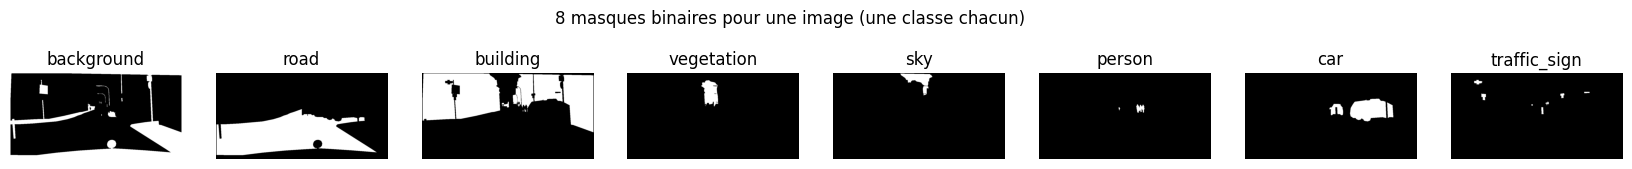
\includegraphics[width=\dimexpr\textwidth-2\fboxsep\relax]{img/masques_binaires.png}}
\setsource{figure du notebook, section 2.6}
\note{(≈ 1 min) Le premier changement est la formulation du problème. La baseline produit 9 cartes de scores et prend, pour chaque pixel, la classe de score maximal~: plus d'un demi-million de décisions indépendantes. Mask2Former et EoMT prédisent un ensemble fixe de N paires~: un vecteur de probabilités p sur les 9 classes plus une classe «~aucun objet~», et un masque binaire m, en logits, au quart de la résolution. Pour revenir à une carte par pixel, on somme pour chaque classe les masques pondérés par leur probabilité, puis on prend le maximum. Côté données, chaque annotation devient un ensemble de masques binaires, un par classe présente~: voici les 8 masques d'une image de validation.}
\end{frame}

%==============================================================
\begin{frame}{Appariement hongrois, puis perte}
\framesubtitle{Démarche · concept 2~: l'apprentissage}
\setsource{Cheng et al., 2022~; Kuhn, 1955}
\vspace{1mm}
\begin{columns}[T,onlytextwidth]
\column{0.46\textwidth}
{\small\bfseries Exemple~: 6 requêtes, 3 classes présentes dans l'image}\par\vspace{2mm}
\begin{tikzpicture}[x=1mm,y=1mm,font=\small]
  \foreach \c/\lab in {0/route,1/voiture,2/personne}{
    \fill[navy, rounded corners=0.5mm] (17+\c*15.5,0) rectangle (17+\c*15.5+14.5,5.2);
    \node[text=paper,font=\small\bfseries] at (17+\c*15.5+7.25,2.6) {\lab};}
  \foreach \r in {1,...,6}{
    \node[anchor=west,font=\small\bfseries] at (0,-\r*5.6+2.4) {requête \r};
    \foreach \c in {0,1,2}{
      \fill[softgrey, rounded corners=0.5mm] (17+\c*15.5,-\r*5.6) rectangle (17+\c*15.5+14.5,-\r*5.6+4.8);}}
  \foreach \r/\c in {1/2,2/0,5/1}{
    \fill[cvgreen, rounded corners=0.5mm] (17+\c*15.5,-\r*5.6) rectangle (17+\c*15.5+14.5,-\r*5.6+4.8);
    \node[text=dkgreen,font=\small\bfseries] at (17+\c*15.5+7.25,-\r*5.6+2.4) {apparié};}
\end{tikzpicture}\par\vspace{2mm}
\soft{\small Requêtes 3, 4 et 6 non appariées~: leur cible devient «~aucun objet~». Chaque masque réel a exactement une requête.}
\column{0.51\textwidth}
\begin{card}[fontupper=\small,before upper={\RaggedRight\abovedisplayskip=3pt\belowdisplayskip=3pt\abovedisplayshortskip=2pt\belowdisplayshortskip=2pt}]
{\bfseries\color{accent}1. Coût de chaque association, puis appariement optimal}
\[\mathcal{C}(j,q) = -2\,p_q(c_j) + 5\,\mathrm{BCE}(m_q, g_j) + 5\,\mathrm{Dice}(m_q, g_j)\]
\[\hat\sigma = \arg\min_{\sigma} \sum_{j=1}^{K} \mathcal{C}\big(j, \sigma(j)\big)\]
{\bfseries\color{accent}2. Perte sur cet appariement, à chaque étape $l$}
\[\mathcal{L} = \sum_{l} \Big[\,2\,\mathcal{L}^{(l)}_{\mathrm{cls}} + 5\,\mathcal{L}^{(l)}_{\mathrm{BCE}} + 5\,\mathcal{L}^{(l)}_{\mathrm{Dice}}\Big]\]
\begin{itemize}\color{bodyc}
\item «~aucun objet~» pondéré 0,1 dans l'entropie croisée
\item supervision profonde~: 10 étapes (Mask2Former), 4 (EoMT)
\end{itemize}
\end{card}
\end{columns}
\note{(≈ 1 min) Comment apprendre un ensemble, alors que l'ordre des requêtes est arbitraire~? Par un appariement. Pour chaque image, on calcule le coût d'associer chaque masque réel à chaque requête~: probabilité de la bonne classe, plus erreur de masque en entropie binaire et en Dice. L'algorithme hongrois trouve l'association de coût total minimal~; dans l'exemple, la requête 2 prend la route, la 5 la voiture, la 1 la personne. Les autres doivent prédire «~aucun objet~». La perte est calculée sur cet appariement, avec les poids de l'article~: 2 pour la classe, 5 pour la BCE et 5 pour le Dice. Les masques sont évalués sur 12\,544 points, choisis surtout là où le modèle hésite, et la perte est appliquée à chaque étape du décodeur~: supervision profonde.}
\end{frame}

%==============================================================
\begin{frame}{L'attention masquée}
\framesubtitle{Démarche · concept 3~: Mask2Former}
\setsource{Cheng et al., CVPR 2022}
\vspace{1mm}
\begin{columns}[T,onlytextwidth]
\column{0.60\textwidth}
\begin{darkcard}
\[X_l = \mathrm{softmax}\Big(\mathcal{M}_{l-1} + \frac{Q_l K_l^{\top}}{\sqrt{d}}\Big)\, V_l + X_{l-1}\]
\[\mathcal{M}_{l-1}(q,x) = \begin{cases} 0 & \text{si } \sigma\big(m_q^{(l-1)}(x)\big) \ge 0{,}5\\[1mm] -\infty & \text{sinon}\end{cases}\]
{\small\color{palegrey}Chaque requête ne regarde que les pixels de son masque prédit à la couche précédente~: le masque s'affine de couche en couche, l'apprentissage converge plus vite.}
\end{darkcard}
\column{0.37\textwidth}
\begin{tikzpicture}[x=1mm,y=1mm]
  \foreach \x in {0,...,7}{\foreach \y in {0,...,3}{
    \fill[cellgrey, rounded corners=0.3mm] (\x*5.2,-\y*5.2) rectangle (\x*5.2+4.7,-\y*5.2+4.7);}}
  \foreach \x/\y in {2/1,3/1,4/1,1/2,2/2,3/2,4/2,5/2,1/3,2/3,3/3,4/3}{
    \fill[cvorange, rounded corners=0.3mm] (\x*5.2,-\y*5.2) rectangle (\x*5.2+4.7,-\y*5.2+4.7);}
\end{tikzpicture}\par\vspace{2mm}
{\small\textbf{\color{dkorange}Orange}~: masque courant de la requête, attention autorisée. \textbf{Gris}~: $-\infty$, ignoré.}
\end{columns}
\vspace{2.5mm}
\begin{tikzpicture}[x=1mm,y=1mm,font=\small,
  box/.style={draw=linec, fill=white, rounded corners=1.2mm, text width=25mm, minimum height=11mm, align=left, inner sep=1.8mm},
  arr/.style={-{Latex[length=2.2mm]}, line width=1.2pt, navy}]
  \node[box] (a) {\textbf{Swin-Tiny}~: cartes à 1/4, 1/8, 1/16, 1/32};
  \node[box, right=5mm of a] (b) {\textbf{Pixel decoder}~: 6 couches d'attention déformable};
  \node[box, right=5mm of b, fill=orangetint, draw=cvorange, text width=30mm] (c) {\textbf{Décodeur}~: 9 couches, 100 requêtes, échelles 1/32, 1/16, 1/8};
  \node[box, right=5mm of c] (d) {\textbf{Masques}~: requête $\cdot$ pixel, à 1/4};
  \draw[arr] (a) -- (b); \draw[arr] (b) -- (c); \draw[arr] (c) -- (d);
\end{tikzpicture}
\note{(≈ 45 s) La nouveauté de Mask2Former est l'attention masquée. Dans l'attention croisée classique, chaque requête regarde toute l'image. Ici, on ajoute un masque M~: zéro là où le masque prédit à la couche précédente dépasse 0,5, moins l'infini ailleurs. Après le softmax, la requête ne regarde que sa propre zone, en orange sur le schéma. Le reste de l'architecture~: un backbone Swin-Tiny, un pixel decoder à attention déformable multi-échelle, et un décodeur de 9 couches qui parcourt les échelles 1/32, 1/16 et 1/8 en boucle. Les masques finaux sont le produit scalaire entre chaque requête et chaque pixel, au quart de la résolution.}
\end{frame}

%==============================================================
\begin{frame}{Un ViT encodeur seul, sans décodeur}
\framesubtitle{Démarche · concept 4~: EoMT}
\setsource{Kerssies et al., 2025}
\vspace{1mm}
\begin{tikzpicture}[x=1mm,y=1mm,font=\small,
  arr/.style={-{Latex[length=2.2mm]}, line width=1.2pt, navy}]
  \node[draw=linec, fill=white, rounded corners=1.2mm, text width=24mm, align=left, inner sep=2mm, minimum height=12mm] (in) at (13,0)
    {\textbf{Entrée}~: 2\,048 patchs 16\,$\times$\,16, CLS, 4~registres};
  \foreach \i in {1,...,12}{
    \pgfmathsetmacro{\xx}{31+(\i-1)*7.3}
    \ifnum\i>9
      \fill[cvgreen, rounded corners=0.8mm] (\xx,-6) rectangle (\xx+6.6,6);
      \node[font=\small\bfseries, text=dkgreen] at (\xx+3.3,0) {\i};
    \else
      \fill[cellgrey, rounded corners=0.8mm] (\xx,-6) rectangle (\xx+6.6,6);
      \node[font=\small\bfseries] at (\xx+3.3,0) {\i};
    \fi}
  \draw[arr] (in.east) -- (30.5,0);
  \draw[arr] (118.4,0) -- (121.4,0);
  \node[draw=cvgreen, fill=greentint, line width=0.8pt, rounded corners=1.2mm, text width=12.5mm, align=center, inner sep=1mm, minimum height=12mm] at (129.8,0) {\textbf{Masques}};
  \node[font=\small\bfseries, text=accent] at (107.3,11) {+ 200 requêtes};
  \draw[arr, accent] (107.3,8.5) -- (107.3,6.5);
\end{tikzpicture}\par\vspace{1mm}
\soft{\small Gris~: blocs ViT-B pré-entraînés DINOv2 \textperiodcentered\ vert~: requêtes et patchs ensemble dans l'auto-attention}\par\vspace{2mm}
\begin{columns}[T,onlytextwidth]
\column{0.32\textwidth}
\begin{card}[equal height group=eomt]\cardtitle{Module de masques}
\vspace{-3mm}
\[\mathbf{p}_n = \mathrm{softmax}\big(W\mathbf{q}_n\big)\]
\vspace{-4mm}
\[m_n = \big\langle \mathrm{MLP}_3(\mathbf{q}_n),\; \mathcal{U}(T)\big\rangle\]
\soft{\small $\mathcal{U}$~: 2 convolutions transposées (1/16 vers 1/4)}
\end{card}
\column{0.32\textwidth}
\begin{card}[equal height group=eomt]\cardtitle{Pourquoi plus rapide}
\begin{itemize}\small\color{bodyc}\setlength{\itemsep}{1mm}
\item aucun décodeur
\item uniquement des opérations de ViT, rapides en bf16
\item aucun masque à calculer à l'inférence
\end{itemize}\end{card}
\column{0.32\textwidth}
\begin{card}[equal height group=eomt]\cardtitle{Adapté au 512\,$\times$\,1024}\vspace{-0.5mm}
\soft{\small Modèle COCO en 640\,$\times$\,640 (grille 40\,$\times$\,40)~: position embeddings interpolées en bicubique vers 32\,$\times$\,64.}
\end{card}
\end{columns}
\note{(≈ 1 min) EoMT supprime tout ce que Mask2Former ajoute autour du backbone. L'image est découpée en 2\,048 patchs de 16 pixels, plus un jeton CLS et 4 registres, et passe dans un ViT-B pré-entraîné avec DINOv2. Avant le dixième bloc, on ajoute 200 requêtes~: dans les trois derniers blocs, requêtes et patchs se mélangent par simple auto-attention. Un petit module produit la classe de chaque requête et son masque, produit scalaire avec les patchs remis au quart de la résolution. Il est plus rapide parce qu'il ne fait que des opérations de ViT, très optimisées en demi-précision, et qu'à l'inférence il ne calcule aucun masque intermédiaire. Adaptation propre au projet~: le modèle pré-entraîné attend du 640 par 640~; j'ai interpolé ses position embeddings vers notre grille 32 par 64.}
\end{frame}

%==============================================================
\begin{frame}{Mask annealing~: retirer les masques}
\framesubtitle{Démarche · concept 5~: EoMT}
\setsource{calendrier du dépôt officiel EoMT, mis à l'échelle de nos 14\,880 pas}
\vspace{1mm}
\begin{columns}[T,onlytextwidth]
\column{0.62\textwidth}
{\small\bfseries Probabilité de garder l'attention masquée, par bloc (entraînement réel, 20~époques)}\par\vspace{1mm}
\begin{tikzpicture}
\begin{axis}[width=92mm, height=47mm, xmin=0, xmax=20, ymin=-0.05, ymax=1.08,
  xtick={0,4,8,12,16,20}, ytick={0,0.5,1}, yticklabels={{0},{0,5},{1}}, xlabel={époque},
  axis lines=left, tick label style={font=\small}, label style={font=\small},
  grid=major, major grid style={linec}, every axis plot/.append style={line width=1.6pt},
  legend style={font=\small, draw=none, fill=none, at={(0.98,0.95)}, anchor=north east}, legend cell align=left]
  \addplot[cvgreen!70!navy, domain=0:20, samples=241] {x<4 ? 1 : (x<8 ? (1-(x-4)/4)^0.9 : 0)};
  \addplot[cvblue, dashed, domain=0:20, samples=241] {x<8 ? 1 : (x<12 ? (1-(x-8)/4)^0.9 : 0)};
  \addplot[cvorange, dotted, domain=0:20, samples=241] {x<12 ? 1 : (x<16 ? (1-(x-12)/4)^0.9 : 0)};
  \legend{bloc 10, bloc 11, bloc 12}
\end{axis}
\end{tikzpicture}
\column{0.35\textwidth}
\begin{card}
\[P_b(t) = \Big(1 - \frac{t - t^{s}_b}{t^{e}_b - t^{s}_b}\Big)^{0{,}9}\]
\soft{\small pour $t^{s}_b \le t < t^{e}_b$~; retrait entre les pas 2\,976 et 11\,904 sur 14\,880.}
\end{card}\par\vspace{3mm}
\begin{darkcard}
{\small\textbf{Validation toujours sans masque}, comme en production~: la mIoU monte pendant le retrait (0,835 $\rightarrow$ 0,842).}
\end{darkcard}
\end{columns}
\note{(≈ 45 s) La technique qui rend EoMT rapide~: le mask annealing. Au début de l'entraînement, les trois derniers blocs utilisent l'attention masquée, ce qui aide à apprendre. Puis, bloc par bloc, la probabilité de l'appliquer décroît de 1 à 0 selon une loi polynomiale. Sur mes 14\,880 pas, le bloc 10 la perd entre les époques 4 et 8, le bloc 11 entre 8 et 12, le bloc 12 entre 12 et 16~; les quatre dernières époques sont entièrement sans masque. J'ai validé à chaque époque sans aucun masque, exactement comme en production, et la mIoU a continué de monter pendant le retrait. L'arrêt anticipé était suspendu pendant cette phase.}
\end{frame}

%==============================================================
{\setbeamercolor{background canvas}{bg=paper2}
\begin{frame}{Recette d'entraînement}
\framesubtitle{Démarche · recette d'entraînement}
\setsource{détails et équations~: doc/poc\_mathematical\_models.tex}
\vspace{1mm}
\begin{card}[colframe=white,left=2mm,right=2mm]
\small
\renewcommand{\arraystretch}{1.35}
\begin{tabularx}{\linewidth}{@{}>{\bfseries}p{23mm}>{\raggedright\arraybackslash}p{30mm}>{\raggedright\arraybackslash}X>{\raggedright\arraybackslash}X@{}}
\toprule
Élément & ResNet50-UNet & Mask2Former & EoMT\\
\midrule
Pré-entraînement & encodeur ImageNet & modèle entier ADE20K & modèle entier COCO (ViT DINOv2)\\
Optimiseur & Adam & AdamW, décroissance 0,05 & AdamW, décroissance 0,05\\
Taux & $10^{-4}$ décodeur, $10^{-5}$ encodeur, constant & $10^{-4}$, backbone $10^{-5}$~; warm-up de 250 pas, puis décroissance polynomiale & $10^{-4}\times 0{,}8^{\,11-l}$ pour la couche $l$~; warm-up des têtes puis du ViT\\
Perte & CE + Dice pondérées & appariement + CE, BCE, Dice & idem, une perte par bloc\\
Lot, précision & 4, fp32 & $2\times2$ accumulés, bf16, gradient $\le 0{,}01$ & $2\times2$ accumulés, bf16, gradient $\le 0{,}01$\\
Spécifique & poids de classe de 0,5 à 3 & tête 150 $\rightarrow$ 9 classes & embeddings $40\times40 \rightarrow 32\times64$, mask annealing\\
\bottomrule
\end{tabularx}
\end{card}
\note{(≈ 45 s) La recette complète, sur une seule vue. Chaque modèle garde celle de son article, pour ne pas le désavantager. Pour EoMT, le taux d'apprentissage décroît par couche, d'un facteur 0,8 par bloc en descendant~: les premières couches du ViT, déjà bien pré-entraînées, bougent peu~; et le warm-up se fait en deux temps, d'abord les têtes avec le ViT gelé, puis le ViT. Pour les deux transformers, la contrainte de 8 Go de GPU est gérée par des lots de 2 avec accumulation de gradient et la demi-précision bf16.}
\end{frame}
}

%==============================================================
{\setbeamercolor{background canvas}{bg=paper2}
\begin{frame}{EoMT~: +0,027 de mIoU}
\framesubtitle{Résultats}
\vspace{0.5mm}
\begin{columns}[T,onlytextwidth]
\column{0.31\textwidth}
\begin{card}[colframe=white,borderline north={1.6mm}{0pt}{cvblue},equal height group=res,top=4mm]
{\small\bfseries\color{bodyc}ResNet50-UNet \textperiodcentered\ baseline}\par\vspace{3mm}
\hugenum{0,816}\par\vspace{1mm}\soft{mIoU validation}\par\vfill
\soft{erreur restante 0,184}
\end{card}
\column{0.31\textwidth}
\begin{card}[colframe=white,borderline north={1.6mm}{0pt}{cvorange},equal height group=res,top=4mm]
{\small\bfseries\color{bodyc}Mask2Former}\par\vspace{3mm}
\hugenum{0,842}\par\vspace{1mm}\soft{mIoU validation}\par\vfill
\textbf{+0,026 vs baseline}\par\soft{erreur restante $-$14~\%}
\end{card}
\column{0.31\textwidth}
\begin{darkcard}[borderline north={1.6mm}{0pt}{cvgreen},equal height group=res,top=4mm]
{\small\bfseries\color{paleblue}EoMT \textperiodcentered\ nouvelle méthode}\par\vspace{3mm}
\hugenum{0,843}\par\vspace{1mm}{\color{paleblue}mIoU validation}\par\vfill
{\bfseries\color{mint}+0,027 vs baseline}\par{\color{paleblue}erreur restante $-$15~\%}
\end{darkcard}
\end{columns}
\vspace{3mm}
\begin{card}[colframe=white]\small\textbf{Lecture~:} à ce niveau, chaque point coûte cher. La baseline laisse 0,184 d'erreur, EoMT 0,157~: \textbf{15~\% de l'erreur restante en moins}. Sur les classes difficiles, davantage~: fond $-$29~\%, personnes $-$15~\%.\end{card}\par\vspace{2mm}
\soft{\small 500 images de validation Cityscapes, 9 classes, 512\,$\times$\,1024 \textperiodcentered\ les trois modèles ré-évalués par le même script}
\note{(≈ 45 s) Le résultat principal. Sur les 500 images de validation, la baseline obtient 0,816 de mIoU, Mask2Former 0,842 et EoMT 0,843. Les deux nouvelles méthodes gagnent environ 2,7 points de mIoU. Dit autrement~: la baseline laisse 18,4 points d'erreur, EoMT 15,7~; EoMT supprime 15~\% de l'erreur restante, et même 29~\% sur la classe fond. À ce niveau, c'est important~: la baseline avait déjà été optimisée parmi cinq architectures CNN. Les trois modèles sont ré-évalués par le même script, avec la même métrique. Valeurs exactes~: 0,8157, 0,8419 et 0,8426.}
\end{frame}
}

%==============================================================
\begin{frame}{Gains sur les classes difficiles}
\framesubtitle{Résultats · par classe}
\setsource{IoU sur les 500 images de validation}
\vspace{1mm}
\begin{columns}[T,onlytextwidth]
\column{0.64\textwidth}
\small
\renewcommand{\arraystretch}{1.25}
\begin{tabular}{@{}lrrrr@{}}
\toprule
\textbf{IoU par classe} & \textbf{Baseline} & \textbf{Mask2Former} & \textbf{EoMT} & \textbf{Gain EoMT}\\
\midrule
\rowcolor{orangetint} fond & 0,755 & 0,813 & 0,827 & +0,071\\
\rowcolor{orangetint} personne & 0,728 & 0,769 & 0,770 & +0,042\\
bâtiment & 0,860 & 0,892 & 0,893 & +0,032\\
\rowcolor{orangetint} panneau & 0,653 & 0,698 & 0,680 & +0,027\\
\rowcolor{orangetint} vélo & 0,691 & 0,713 & 0,718 & +0,027\\
route & 0,926 & 0,946 & 0,953 & +0,027\\
voiture & 0,914 & 0,930 & 0,934 & +0,020\\
végétation & 0,895 & 0,903 & 0,902 & +0,007\\
ciel & 0,918 & 0,912 & 0,907 & $-$0,011\\
\bottomrule
\end{tabular}
\column{0.33\textwidth}
\begin{card}\small\textbf{Lignes surlignées}~: les classes rares ou hétérogènes, où la baseline était faible.\end{card}\par\vspace{2.5mm}
\begin{card}\small\textbf{8 classes sur 9 progressent}, toutes de façon significative (bootstrap).\end{card}\par\vspace{2.5mm}
\begin{card}\small\textbf{Seule baisse~: le ciel} ($-$0,011), grande zone simple déjà bien traitée.\end{card}
\end{columns}
\note{(≈ 45 s) Le détail par classe confirme l'hypothèse du plan prévisionnel. Les gains les plus nets sont sur le fond, qui regroupe des éléments très variés, sur les personnes (+0,042) et sur les panneaux et les vélos (+0,027)~: les petits objets où la baseline était faible. Huit classes sur neuf progressent, toutes de façon significative selon le bootstrap. La seule baisse est le ciel, une grande zone homogène déjà très bien traitée. Mask2Former est légèrement meilleur qu'EoMT sur les panneaux.}
\end{frame}

%==============================================================
\begin{frame}{Même précision, 2,4\,$\times$ plus rapide}
\framesubtitle{Résultats · vitesse}
\setsource{seuls les rapports entre modèles se transposent à un autre matériel}
\vspace{1mm}
{\small\bfseries Temps d'inférence d'une image 512\,$\times$\,1024 \textperiodcentered\ GPU portable RTX 2000 Ada, bf16}\par\vspace{3mm}
\begin{tikzpicture}[x=1mm,y=1mm,font=\normalsize]
  \foreach \lab/\ms/\col/\txt/\i in {ResNet50-UNet/19/cvblue/{19 ms \textperiodcentered\ 41 M param.}/0,
                                     Mask2Former/106/cvorange/{106 ms \textperiodcentered\ 47 M}/1,
                                     EoMT/43/cvgreen/{43 ms \textperiodcentered\ 94 M}/2}{
    \fill[\col, rounded corners=0.6mm] (0,-\i*8.5) rectangle (\ms*0.62,-\i*8.5+5.5);
    \node[anchor=east] at (-2,-\i*8.5+2.75) {\lab};
    \node[anchor=west,font=\normalsize\bfseries] at (\ms*0.62+2,-\i*8.5+2.75) {\txt};}
\end{tikzpicture}\par\vspace{3mm}
\begin{columns}[T,onlytextwidth]
\column{0.485\textwidth}
\begin{card}\cardtitle{Le compromis}\soft{EoMT~: même précision que Mask2Former, 2,4\,$\times$ plus rapide. La baseline reste 2\,$\times$ plus rapide qu'EoMT, pour 0,027 de mIoU en moins.}\end{card}
\column{0.485\textwidth}
\begin{card}\cardtitle{Sur CPU (cloud)}\soft{Sans GPU ni bf16, l'avantage d'EoMT disparaît~: environ 1,6~s, 3,2~s et 4,1~s par image sur 2~CPU.}\end{card}
\end{columns}
\note{(≈ 45 s) Côté vitesse, sur mon GPU en précision bf16~: 19 millisecondes pour la baseline, 106 pour Mask2Former, 43 pour EoMT. EoMT atteint la précision de Mask2Former en étant 2,4 fois plus rapide, ce qui confirme l'argument de l'article sur un autre jeu et une autre résolution. Deux nuances~: la baseline reste deux fois plus rapide qu'EoMT~; et sur CPU, comme sur le dashboard gratuit, l'avantage disparaît car il repose sur les c\oe urs tensoriels du GPU en demi-précision.}
\end{frame}

%==============================================================
{\setbeamercolor{background canvas}{bg=paper2}
\begin{frame}{Des écarts réels et reproductibles}
\framesubtitle{Résultats · fiabilité}
\vspace{2mm}
\begin{columns}[T,onlytextwidth]
\column{0.56\textwidth}
\begin{card}[colframe=white,equal height group=robust]\cardtitle{Bootstrap apparié, 2\,000 tirages}
\footnotesize\renewcommand{\arraystretch}{1.3}
\begin{tabular}{@{}lrcl@{}}
\toprule
\textbf{Écart de mIoU} & $\Delta$ & \textbf{IC 95~\%} & \textbf{Verdict}\\
\midrule
Mask2Former $-$ base & +0,026 & [0,021~; 0,031] & réel\\
EoMT $-$ base & +0,027 & [0,022~; 0,032] & réel\\
EoMT $-$ Mask2Former & +0,001 & [$-$0,003~; 0,005] & égalité\\
\bottomrule
\end{tabular}\par\vspace{3mm}
\soft{On ré-échantillonne 2\,000 fois les 500 images de validation (tirage avec remise)~: l'écart avec la baseline reste toujours positif.}
\end{card}
\column{0.41\textwidth}
\begin{card}[colframe=white,equal height group=robust]\cardtitle{Ré-entraînement complet}
\small\renewcommand{\arraystretch}{1.3}
\begin{tabular}{@{}lrr@{}}
\toprule
\textbf{mIoU} & \textbf{Notebook} & \textbf{Référence}\\
\midrule
ResNet50-UNet & 0,8152 & 0,8157\\
Mask2Former & 0,8402 & 0,8419\\
EoMT & 0,8423 & 0,8426\\
\bottomrule
\end{tabular}\par\vspace{3mm}
\soft{Les trois modèles ré-entraînés de zéro dans le notebook~: écarts inférieurs à 0,002.}
\end{card}
\end{columns}
\note{(≈ 1 min) Deux vérifications de fiabilité. À gauche, le bootstrap apparié~: on ré-échantillonne 2\,000 fois les images de validation et on recalcule l'écart. L'intervalle à 95~\% de l'écart avec la baseline est entièrement positif, pour Mask2Former comme pour EoMT~: le gain ne dépend pas des images choisies. Entre EoMT et Mask2Former, l'intervalle contient zéro~: égalité en précision. À droite, la reproductibilité~: j'ai ré-entraîné les trois modèles de zéro dans le notebook livré~; les résultats diffèrent de moins de 0,002 des entraînements de référence.}
\end{frame}
}

%==============================================================
\begin{frame}{Contours plus nets, moins de bruit}
\framesubtitle{Résultats · exemples}
\setsource{figure du notebook, section 7.4}
\vspace{1mm}
\colorbox{white}{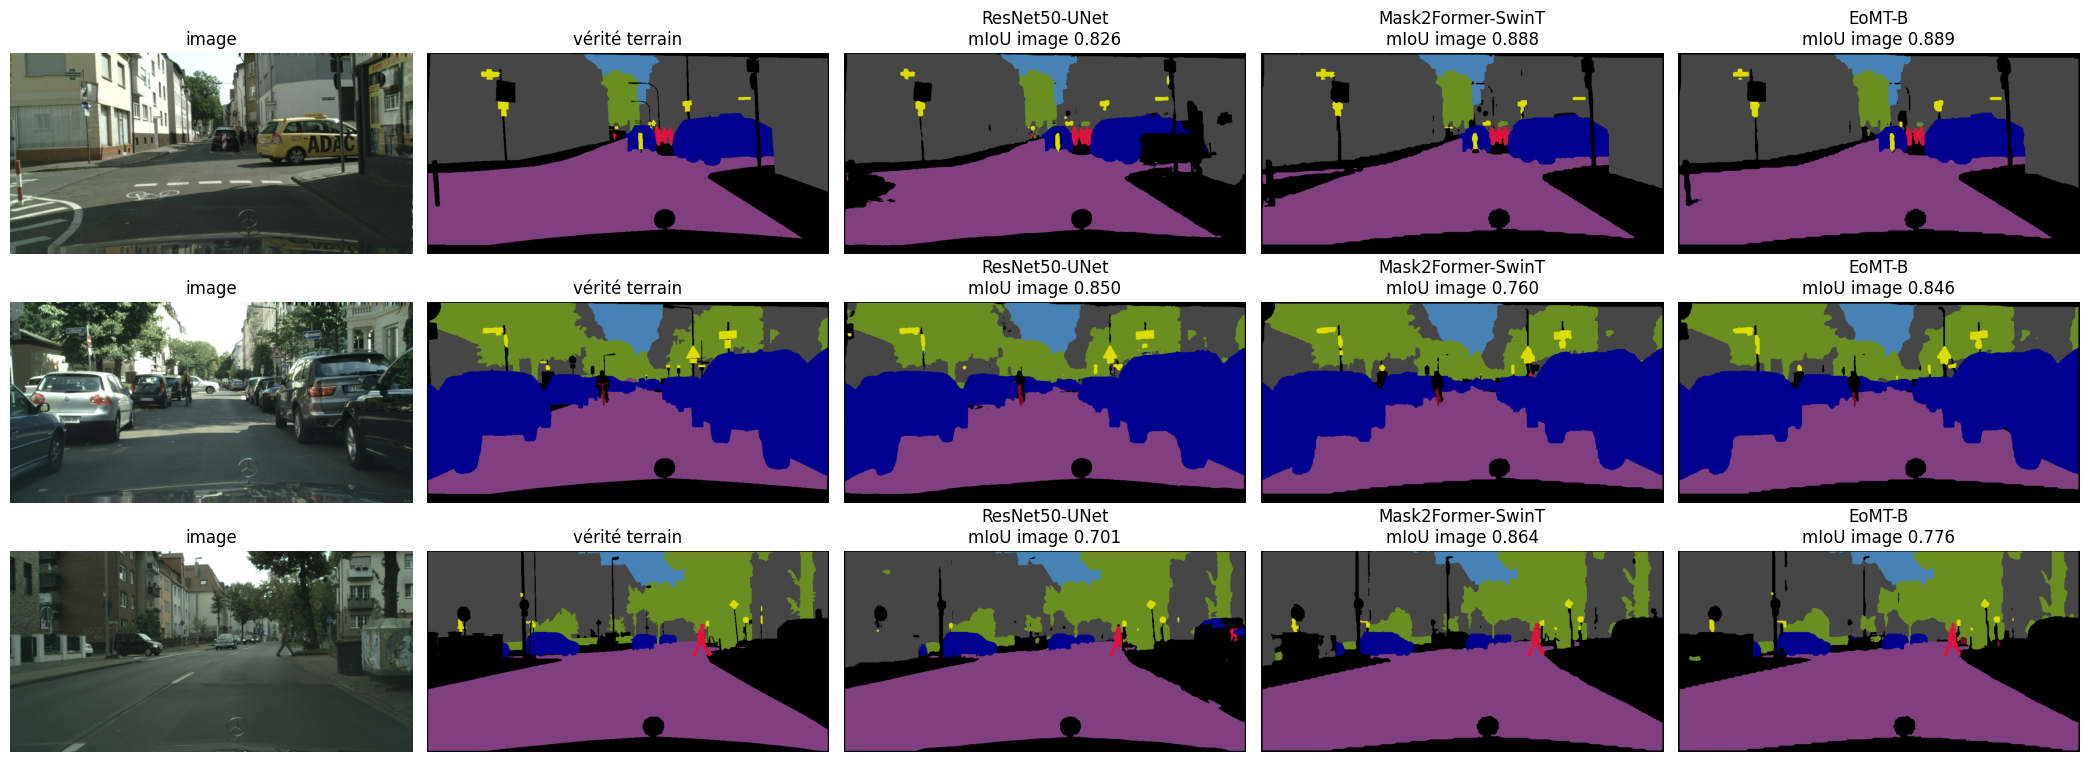
\includegraphics[width=\dimexpr\textwidth-2\fboxsep\relax]{img/predictions.png}}\par\vspace{2mm}
\soft{Colonnes~: image, vérité terrain, ResNet50-UNet, Mask2Former, EoMT. La mIoU d'une seule image varie beaucoup~: les conclusions viennent des 500 images.}
\note{(≈ 30 s) Trois exemples tirés du notebook. Sur la première image, la baseline produit des taches de fond parasites au bord de la route et autour des voitures~; les deux transformers rendent des contours plus propres. Les petits objets, panneaux en jaune et piéton en rouge, sont trouvés par tous, mais mieux formés par les transformers. Sur une seule image, le classement peut s'inverser, par exemple Mask2Former est moins bon sur la deuxième~: c'est pourquoi les conclusions reposent sur les 500 images et sur le bootstrap.}
\end{frame}

%==============================================================
\begin{frame}{Limites de la méthode, pistes d'amélioration}
\framesubtitle{Résultats · la méthode EoMT}
\setsource{mesures du projet~; hypothèses signalées}
\vspace{1mm}
\begin{columns}[T,onlytextwidth]
\column{0.485\textwidth}
\begin{card}[equal height group=meth]\cardtitle{Limites d'EoMT}
\begin{itemize}\small\color{bodyc}\setlength{\itemsep}{0.8mm}
\item \textbf{Dépend du pré-entraînement}~: sans ViT pré-entraîné (DINOv2), aucun décodeur ne compense
\item \textbf{Lourd}~: 94\,M paramètres (baseline 41\,M)
\item \textbf{Coût quadratique}~: en pleine résolution, 4\,$\times$ plus de patchs, $\approx$\,16\,$\times$ plus d'attention
\item \textbf{Rapide seulement sur GPU}~: sur CPU, 4,1~s contre 1,6~s (baseline)
\item \textbf{Petits objets}~: panneaux 0,680, vélos 0,718~; panneaux sous Mask2Former (COCO~? hypothèse)
\end{itemize}\end{card}
\column{0.485\textwidth}
\begin{card}[equal height group=meth]\cardtitle{Pistes d'amélioration}
\begin{itemize}\small\color{bodyc}\setlength{\itemsep}{0.8mm}
\item \textbf{Résolution native}~: un Mask2Former Cityscapes passe de 0,708 à 0,742 (test sur 10 images)
\item \textbf{Augmentation} de l'article~: échelles, recadrages, retournements
\item \textbf{Plus long}~: 20 époques seulement ici
\item \textbf{ViT-L} au lieu de ViT-B (GPU plus grand)
\item \textbf{Sans ré-entraîner}~: augmentation au test (retournement, multi-échelle)
\end{itemize}\end{card}
\end{columns}
\note{(≈ 45 s) Les limites de la méthode elle-même. EoMT supprime le décodeur et s'appuie entièrement sur un ViT pré-entraîné à grande échelle~: sans un tel point de départ, la méthode perd son intérêt. Le modèle est lourd, 94 millions de paramètres. L'attention est quadratique en nombre de tokens~: en pleine résolution, quatre fois plus de patchs, environ seize fois plus de calcul d'attention. La vitesse n'existe que sur GPU en demi-précision. Et les petits objets restent les plus faibles~; sur les panneaux, EoMT est sous Mask2Former, sans doute à cause du pré-entraînement COCO, mais c'est une hypothèse. Pistes~: la résolution native, qui est le levier principal pour les petits objets, notre test préalable le montre~; l'augmentation de données de l'article~; un entraînement plus long~; un ViT plus grand~; et, sans ré-entraîner, l'augmentation au moment du test.}
\end{frame}

%==============================================================
\begin{frame}{Limites de l'étude et suites}
\framesubtitle{Résultats · limites et suites}
\vspace{2mm}
\begin{columns}[T,onlytextwidth]
\column{0.485\textwidth}
\begin{card}[equal height group=lim]\cardtitle{Limites}
\begin{itemize}\color{bodyc}\setlength{\itemsep}{1.2mm}
\item La validation sert à choisir l'époque et à mesurer~: scores un peu optimistes, pour les trois modèles
\item Pas d'augmentation de données~: sur-apprentissage modéré (écart train $-$ validation de +0,06 à +0,08)
\item Points de départ pré-entraînés différents d'un modèle à l'autre
\item Sans GPU, EoMT perd son avantage de vitesse
\end{itemize}\end{card}
\column{0.485\textwidth}
\begin{card}[equal height group=lim]\cardtitle{Suites proposées}
\begin{itemize}\color{bodyc}\setlength{\itemsep}{1.2mm}
\item Plusieurs entraînements par modèle pour mesurer la variance
\item Servir EoMT par l'API du projet, sur une machine avec GPU
\item Quantification ou distillation pour un usage sur CPU
\item Évaluer sur le jeu de test officiel via le serveur Cityscapes
\end{itemize}\end{card}
\end{columns}
\note{(≈ 45 s) Les limites de l'étude, honnêtement. La validation sert à la fois à choisir la meilleure époque et à mesurer~: scores légèrement optimistes, mais de la même façon pour les trois modèles. Aucun modèle n'a d'augmentation de données, et les transformers sur-apprennent un peu. Les points de départ pré-entraînés diffèrent, c'est inhérent à chaque méthode. Et sans GPU, l'avantage de vitesse d'EoMT disparaît. Suites naturelles~: plusieurs entraînements par modèle pour mesurer la variance, servir EoMT par l'API sur une machine GPU, quantifier le modèle pour le CPU, et évaluer sur le jeu de test officiel.}
\end{frame}

%==============================================================
{\setbeamercolor{background canvas}{bg=paper2}
\begin{frame}{Le dashboard, déployé sur le cloud}
\framesubtitle{Démonstration}
\setsource{Streamlit, 3 modèles exécutés sur CPU dans un Space Hugging Face}
\vspace{1mm}
\begin{columns}[T,onlytextwidth]
\column{0.40\textwidth}
{\footnotesize\bfseries\color{accent}\href{https://huggingface.co/spaces/DaryaEL/cityvision-poc}{huggingface.co/spaces/DaryaEL/cityvision-poc}}\par\vspace{3mm}
\begin{enumerate}\small\setlength{\itemsep}{1mm}
\item \textbf{Dataset}~: comptages, exemples par ville et par classe, égalisation, CLAHE, flou
\item \textbf{Prediction}~: choix d'une image et d'un modèle, masque prédit et scores
\item \textbf{Model comparison}~: précision, vitesse, bootstrap, courbes
\end{enumerate}\par\vspace{3mm}
\soft{\small Accessibilité (WCAG)~: textes alternatifs, tableau sous chaque graphique, couleurs lisibles par les daltoniens, commandes au clavier.}
\column{0.57\textwidth}
\fcolorbox{linec}{white}{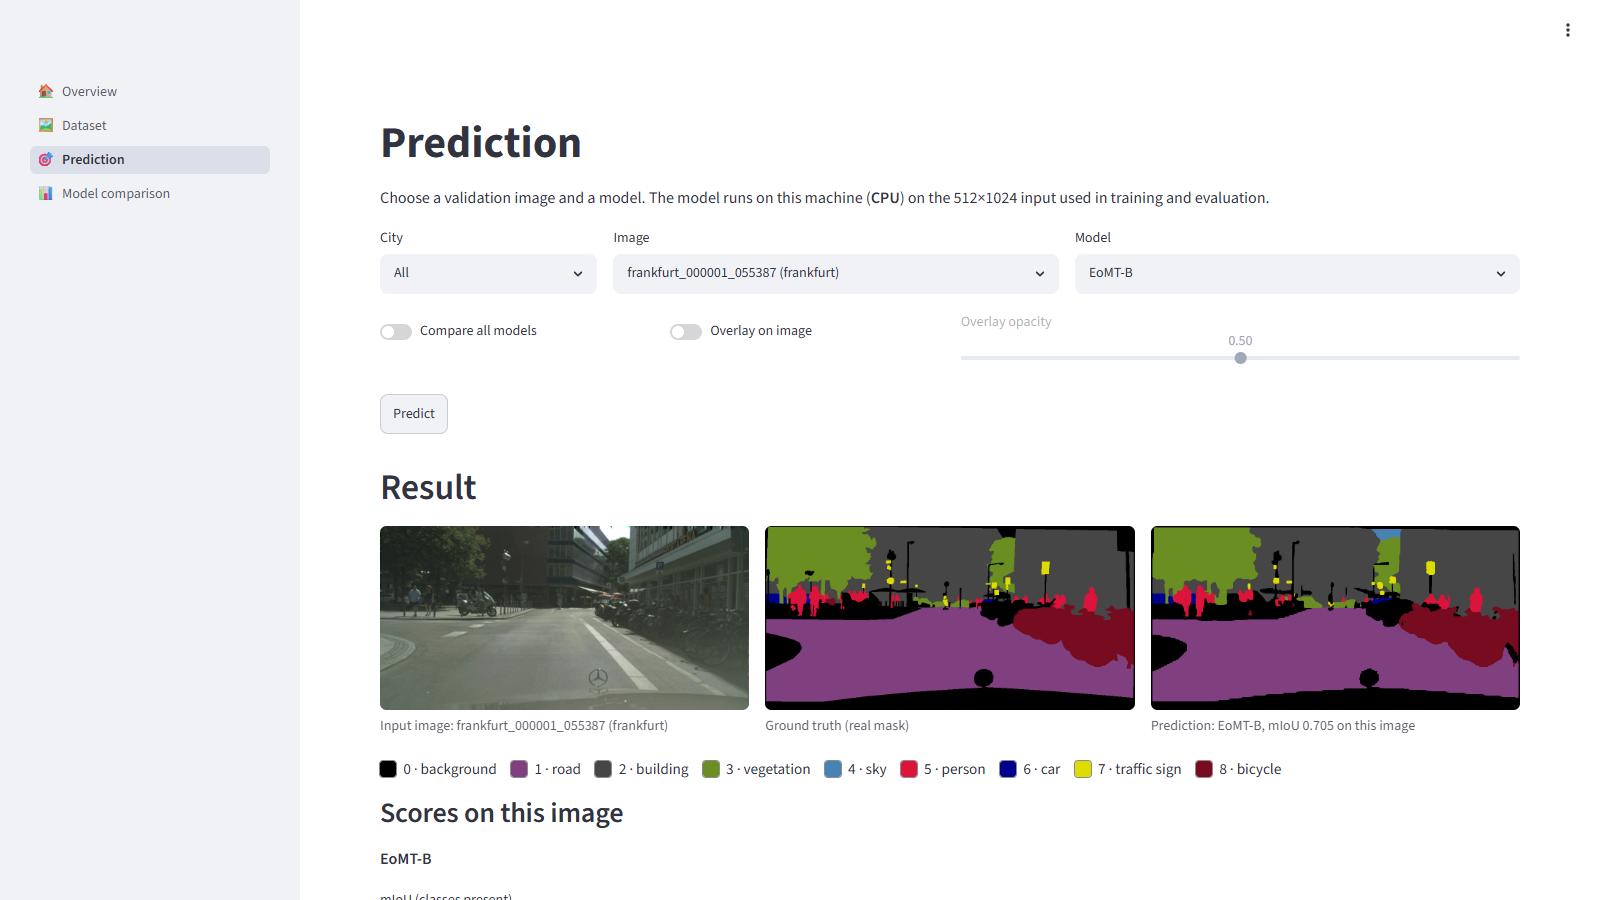
\includegraphics[width=\dimexpr\linewidth-2\fboxsep-0.8pt\relax]{img/demo_prediction.png}}
\end{columns}
\note{(≈ 4 min 30, démo en direct) Avant la présentation~: ouvrir le dashboard quelques minutes à l'avance pour le réveiller (Space gratuit). 1) Page Dataset~: comptages par ville et par classe, galerie par classe (choisir «~bicycle~»), puis une transformation~: CLAHE avec le curseur, et l'histogramme avant / après. 2) Page Prediction~: choisir une image, modèle EoMT, cliquer Predict~; commenter le masque prédit face au vrai masque et le tableau par classe~; puis activer «~Compare all models~» pour voir les trois côte à côte (environ 10 s sur CPU). 3) Page Model comparison~: le graphique précision / vitesse et les intervalles du bootstrap. Mentionner l'accessibilité~: chaque image a un texte alternatif, chaque graphique un tableau. En cas de problème réseau, cette capture sert de secours.}
\end{frame}
}

%==============================================================
{\setbeamercolor{background canvas}{bg=navy}
\begin{frame}[plain,c]
\begin{tikzpicture}[remember picture,overlay]
  \fill[cvblue]   (current page.north west) rectangle ([xshift=53.33mm,yshift=-1.4mm]current page.north west);
  \fill[cvorange] ([xshift=53.33mm]current page.north west) rectangle ([xshift=106.67mm,yshift=-1.4mm]current page.north west);
  \fill[cvgreen]  ([xshift=106.67mm]current page.north west) rectangle ([yshift=-1.4mm]current page.north east);
\end{tikzpicture}
{\fontsize{8}{10}\selectfont\bfseries\color{mint}CONCLUSION}\par\vspace{4mm}
{\fontsize{21}{27}\selectfont\bfseries\color{paper}EoMT bat la baseline\\et égale Mask2Former, en plus rapide\par}\vspace{7mm}
\begin{columns}[T,onlytextwidth]
\column{0.31\textwidth}
\begin{statbox}[cvgreen]{\fontsize{20}{22}\selectfont\bfseries\color{paper}+0,027}\par{\color{paleblue}de mIoU sur la baseline, significatif}\end{statbox}
\column{0.31\textwidth}
\begin{statbox}[cvgreen]{\fontsize{20}{22}\selectfont\bfseries\color{paper}2,4\,$\times$}\par{\color{paleblue}plus rapide que Mask2Former sur GPU}\end{statbox}
\column{0.31\textwidth}
\begin{statbox}[cvgreen]{\fontsize{20}{22}\selectfont\bfseries\color{paper}$-$15~\%}\par{\color{paleblue}d'erreur restante (1 $-$ mIoU)}\end{statbox}
\end{columns}
\vspace{9mm}
{\fontsize{14}{17}\selectfont\bfseries\color{mint}Merci. Questions~?}
\note{(≈ 30 s) Pour conclure~: EoMT, un modèle de 2025, améliore la baseline de 2,7 points de mIoU, de façon statistiquement significative~: 15~\% de l'erreur restante en moins, davantage sur les classes difficiles. Il égale Mask2Former en précision tout en étant 2,4 fois plus rapide sur GPU. Un ré-entraînement complet reproduit ces résultats à moins de 0,002 près. Recommandation~: adopter EoMT pour la prochaine version de CityVision, servi sur GPU, avec de l'augmentation de données. Merci, je suis prête pour vos questions.}
\end{frame}
}

\end{document}
